\documentclass{article}

\usepackage{graphicx}
\usepackage{tikz}
\usepackage{tikzsymbols}
\usetikzlibrary{calc,patterns,shapes.geometric}
\pagestyle{empty}
\usepackage[margin=0pt]{geometry}
\geometry{papersize={14in,12in}}

\def\centerarc[#1](#2)(#3:#4:#5){\draw[#1] ($(#2)+({#5*cos(#3)},{#5*sin(#3)})$) arc (#3:#4:#5);}

\begin{document}
	\begin{figure}
		\centering
		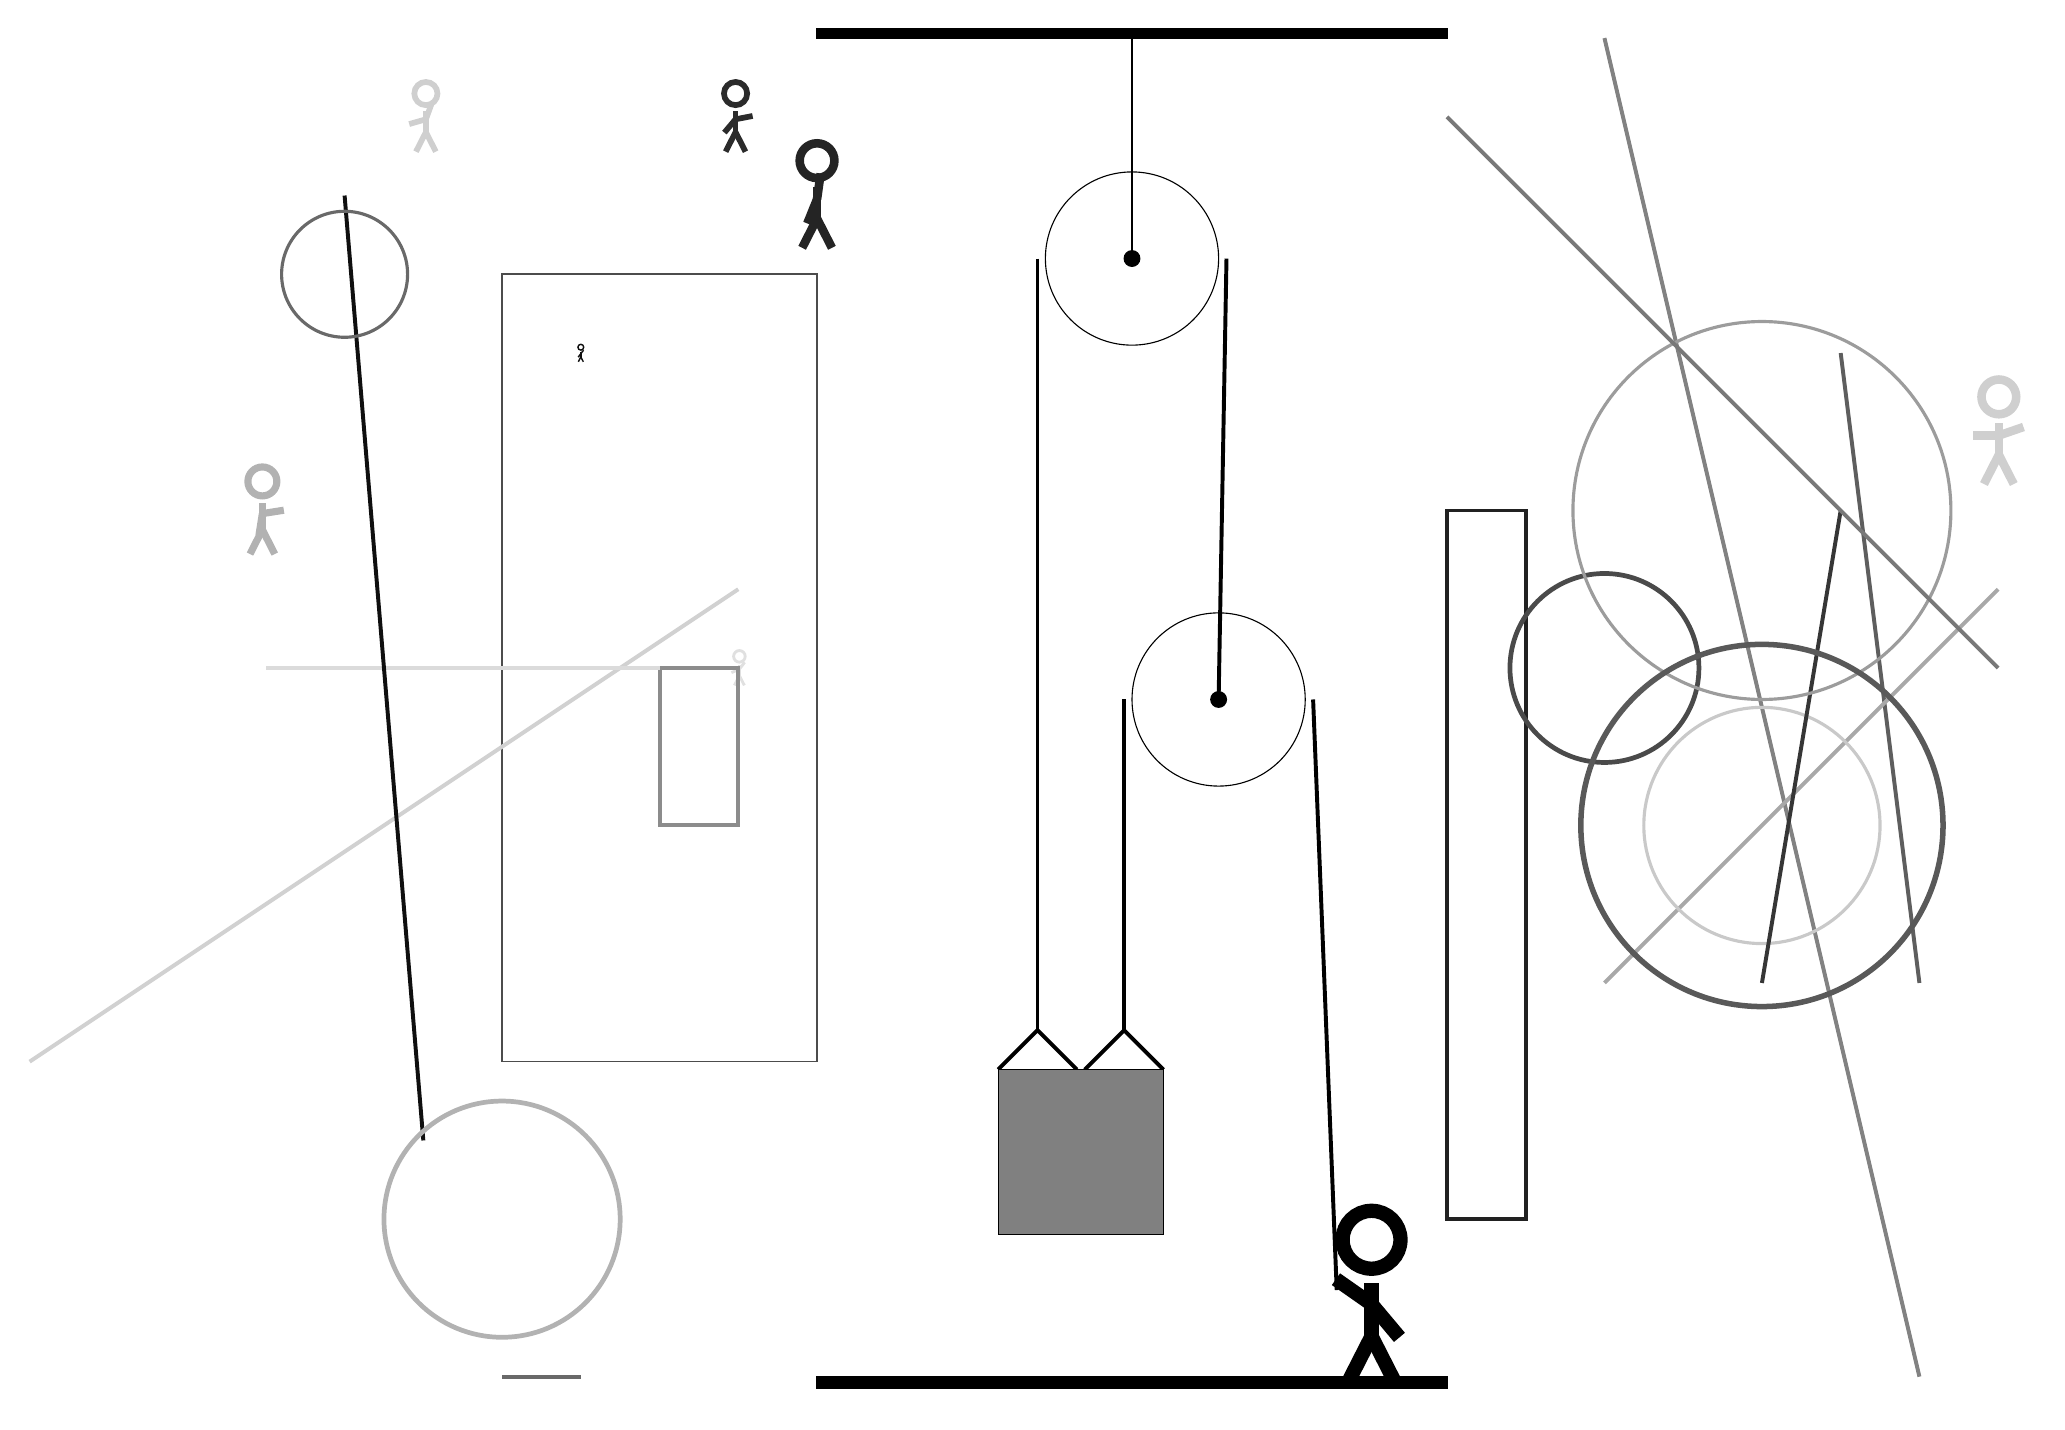
\begin{tikzpicture}
			%%%%% START %%%%%
			
			\draw[fill=black] (-2, 14) rectangle (6, 14.125);
			
			\draw (2, 11.2) circle (1.1);
			\draw[fill=black] (2, 11.2) circle (0.1);
			\draw[thick] (2, 11.2) -- (2, 14);
			
			\draw (3.1, 5.6) circle (1.1);
			\draw[fill=black] (3.1, 5.6) circle (0.1);
			
			\draw[line width = 0.5mm]  (0.3, 0.9) -- (0.8, 1.4) -- (1.3, 0.9);
			\draw[line width = 0.5mm]  (1.4, 0.9) -- (1.9, 1.4) -- (2.4, 0.9);
			\draw[fill=black!50] (0.3, 0.9) rectangle (2.4, -1.2);
			
			\draw[line width = 0.5mm] (0.8, 11.2) -- (0.8, 1.4);
			\centerarc[line width = 0.5mm](2, 11.2)(0:180:1.2000000000000002);
			\draw[line width = 0.5mm] (3.2, 11.2) -- (3.1, 5.6);
			\draw[line width = 0.5mm] (1.9, 5.6) -- (1.9, 1.4);
			\centerarc[line width = 0.5mm](3.1, 5.6)(0:180:1.2000000000000002);
			\draw[line width = 0.5mm] (4.3, 5.6) -- (4.6, -1.9);
			
			\node at (5, -2) {\Strichmaxerl[10][-35][-50]};
			
			\draw[line width=0.5mm, color=black!63](11, 10) -- (12, 2);
			
			\draw[line width=0.5mm, color=black!49](8, 14) -- (12, -3);
			\draw[line width=0.5mm, color=black!59](-6, -3) -- (-5, -3);
			\draw[line width=0.2mm, color=black!70] (-2, 1) rectangle (-6, 11);
			\node[line width=0.2mm, color=black!19] at (13, 9) {\Strichmaxerl[6][0][19]};
			\node[line width=0.3mm, color=black!83] at (-3, 13) {\Strichmaxerl[4][50][11]};
			\node[line width=0.2mm, color=black!86] at (-2, 12) {\Strichmaxerl[6][68][82]};
			\draw[line width=0.5mm, color=black!18](-3, 7) -- (-12, 1);
			\draw[line width=0.5mm, color=black!34](8, 2) -- (13, 7);
			
			\node[line width=0.5mm, color=black!12] at (-3, 6) {\Strichmaxerl[2][23][53]};
			
			\draw[line width=0.5mm, color=black!45] (-4, 4) rectangle (-3, 6);
			\draw[line width=0.5mm, color=black!87] (7, 8) rectangle (6, -1);
			\node[line width=0.3mm, color=black!19] at (-7, 13) {\Strichmaxerl[4][16][70]};
			
			\draw[line width=0.5mm, color=black!14](-4, 6) -- (-9, 6);
			\draw [line width=0.4mm, color=black!21](10, 4) circle (1.5);
			\draw[line width=0.5mm, color=black!94](-7, 0) -- (-8, 12);
			
			\draw [line width=0.4mm, color=black!59](-8, 11) circle (0.8);
			\draw[line width=0.5mm, color=black!79](10, 2) -- (11, 8);
			\node[line width=0.5mm, color=black!94] at (-5, 10) {\Strichmaxerl[1][53][51]};
			\draw [line width=0.6mm, color=black!71](8, 6) circle (1.2);
			\draw [line width=0.4mm, color=black!39](10, 8) circle (2.4);
			
			\draw [line width=0.7mm, color=black!65](10, 4) circle (2.3);
			\node[line width=0.4mm, color=black!30] at (-9, 8) {\Strichmaxerl[5][81][9]};
			\draw [line width=0.6mm, color=black!30](-6, -1) circle (1.5);
			\draw[line width=0.5mm, color=black!53](6, 13) -- (13, 6);
			
			\draw[fill=black] (-2, -3) rectangle (6, -3.15);
			
			%%%%% END %%%%%
		\end{tikzpicture}
	\end{figure}	
\end{document}